\documentclass[a4paper,14pt]{extarticle}

\usepackage[utf8x]{inputenc}
\usepackage[T1,T2A]{fontenc}
\usepackage[russian]{babel}
\usepackage{hyperref}
\usepackage{indentfirst}
\usepackage{here}
\usepackage{array}
\usepackage{graphicx}
\usepackage{caption}
\usepackage{subcaption}
\usepackage{chngcntr}
\usepackage{amsmath}
\usepackage{amssymb}
\usepackage{pgfplots}
\usepackage{pgfplotstable}
\usepackage[left=2cm,right=2cm,top=2cm,bottom=2cm,bindingoffset=0cm]{geometry}
\usepackage{multicol}
\usepackage{askmaps}
\usepackage{titlesec}
\usepackage{listings}
\usepackage{color}
\usepackage{courier}

\definecolor{green}{rgb}{0,0.6,0}
\definecolor{gray}{rgb}{0.5,0.5,0.5}
\definecolor{purple}{rgb}{0.58,0,0.82}

\lstset{
	language=Verilog,
	backgroundcolor=\color{white},   
	basicstyle=\small\ttfamily,
	commentstyle=\color{green},
	keywordstyle=\color{blue},	
	numberstyle=\tiny\color{gray},
	stringstyle=\color{purple},
	breakatwhitespace=false,
	breaklines=true,
	captionpos=b,
	keepspaces=true,
	numbers=left,
	numbersep=5pt,
	showspaces=false,
	showstringspaces=false,
	showtabs=false,
	tabsize=4,
	frame=single,
	inputpath={../quartus/},
	literate={~} {$\sim$}{1}
}

\renewcommand{\le}{\ensuremath{\leqslant}}
\renewcommand{\leq}{\ensuremath{\leqslant}}
\renewcommand{\ge}{\ensuremath{\geqslant}}
\renewcommand{\geq}{\ensuremath{\geqslant}}
\renewcommand{\epsilon}{\ensuremath{\varepsilon}}
\renewcommand{\phi}{\ensuremath{\varphi}}
\renewcommand{\thefigure}{\arabic{figure}} 	
\renewcommand*\not[1]{\overline{#1}}

\titleformat*{\section}{\large\bfseries} 
\titleformat*{\subsection}{\normalsize\bfseries} 
\titleformat*{\subsubsection}{\normalsize\bfseries} 
\titleformat*{\paragraph}{\normalsize\bfseries} 
\titleformat*{\subparagraph}{\normalsize\bfseries} 

\counterwithin{figure}{section}
\counterwithin{equation}{section}
\counterwithin{table}{section}
\newcommand{\sign}[1][5cm]{\makebox[#1]{\hrulefill}}
\graphicspath{{../pics/}}
\captionsetup{justification=centering,margin=1cm}
\def\arraystretch{1.3}
\setlength\parindent{5ex}
\titlelabel{\thetitle.\quad}

\begin{document}

\begin{titlepage}
\begin{center}
	Санкт-Петербургский Политехнический Университет Петра Великого\\[0.3cm]
	Институт компьютерных наук и технологий \\[0.3cm]
	Кафедра компьютерных систем и программных технологий\\[4cm]
	
	\textbf{ОТЧЕТ}\\ 
	\textbf{по лабораторной работе}\\[0.5cm]
	\textbf{SystemVerilog №4}\\[0.1cm]
	Автоматизация проектирования\\ дискретных устройств\\[4.0cm]
\end{center}

\begin{flushright}
	\begin{minipage}{0.45\textwidth}
		\textbf{Работу выполнил студент}\\[3mm]
		группа 33501/4 \hspace*{9mm} Дьячков В.В.\\[5mm]
		\textbf{Преподаватель}\\[5mm]
		\sign[1.5cm] \hspace*{1mm} к.т.н., доц. Филиппов А.С. \\[5mm]
	\end{minipage}
\end{flushright}

\vfill

\begin{center}
	Санкт-Петербург\\
	\the\year
\end{center}
\end{titlepage}

\addtocounter{page}{1}
\counterwithin{lstlisting}{section}

\tableofcontents
\lstlistoflistings
\listoffigures
\newpage

\section{Задание}

\begin{itemize}
	\item На языке Verilog описать параметризированный преобразователь $N$-разрядного двоичного кода в позиционный код (переключатели платы \code{miniDiLaB_CIV} задают двоичный код; светодиоды отображают позиционный код):
		\begin{itemize}
			\item Модуль -- \code{b2oh}; файл \code{b2oh.v}; проект в Quartus -- \code{b2oh}; \item Рабочая папка -- \code{labs_1};
			\item Параметр $N$ -- разрядность двоичного кода: $N=3$ -- задается из теста (базовое значение параметра -- $8$) стандарты и номера выводов СБИС для платы \code{miniDiLaB_CIV} задать с помощью атрибутов.
		\end{itemize}
	
	\item На языке Verilog создать описание тестов:
		\begin{itemize}
			\item Тест класса 1 -- \code{tb1_b2oh.v};
			\item Тест класса 2 с вычислением результата -- \code{tb2_b2oh.v} (должен обеспечить проверку всех возможных вариантов входных сигналов);
			\item Тест класса 2 с чтением файлов -- \code{tb2f_b2oh.v} (файл с тестовыми воздействиями -- \code{input_b2oh.dat}, файл с ожидаемыми результатами -- \code{exp_b2oh.dat}).
		\end{itemize}
	\item Осуществить моделирование и отладку модулей и проверку тестов класса 2.
	\item Реализовать проект на плате \code{miniDiLaB_CIV}.
\end{itemize}

\section{Описание устройства}

В листинге \ref{code:b2oh} приведено описание параметризированного преобразователя $N$-разрядного двоичного кода в позиционный.
\lstinputlisting[caption=\code{b2oh.v}, label=code:b2oh]{b2oh.v}

\section{Описание тестов}
\label{sec:tests}

\subsection{Тест первого класса}

В листинге \ref{code:test1} приведено описание теста первого класса.
\lstinputlisting[caption=\code{tb1_b2oh.v}, label=code:test1]{tb1_b2oh.v}

В листинге \ref{code:test1_results} приведен вывод результатов теста в консоль.
\begin{lstlisting}[caption=Результаты теста первого класса, label=code:test1_results, style=console]
run -all
# 		          time binary positional
#                    0   0     1
#                  100   1     2
#                  200   2     4
#                  300   3     8
#                  400   4    16
#                  500   5    32
#                  600   6    64
#                  700   7   128
#    Time: 800 ns  Iteration: 0  Instance: /tb1_b2oh
\end{lstlisting}

На рис. \ref{fig:test1_results} изображена временная диаграмма теста.
\begin{figure}[H]
	\begin{center}
		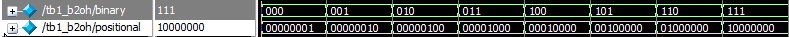
\includegraphics[width=\textwidth]{test1_results}
		\caption{Результаты теста первого класса}
		\label{fig:test1_results}
	\end{center}
\end{figure}
\vspace{-1cm}

\subsection{Тест второго класса с вычислением результата}

В листинге \ref{code:test2} приведено описание теста второго класса с вычислением результата. В данном тесте на вход устройства подаются всевозможные значения преобразуемого кода, а также вычисляется ожидаемое значение результата.
\lstinputlisting[caption=\code{tb2_b2oh.v}, label=code:test2]{tb2_b2oh.v}

В листинге \ref{code:test2_results} приведен вывод результатов теста в консоль.
\begin{lstlisting}[caption=Результаты теста второго класса с вычислением результата, label=code:test2_results, style=console]
run -all
# 		          time binary positional
#                   40   0     1
#                  120   1     2
#                  200   2     4
#                  280   3     8
#                  360   4    16
#                  440   5    32
#                  520   6    64
#                  600   7   128
# Testing complited
#    Time: 640 ns  Iteration: 1  Instance: /tb2_b2oh
\end{lstlisting}

На рис. \ref{fig:test2_results} изображена временная диаграмма теста.
\begin{figure}[H]
	\begin{center}
		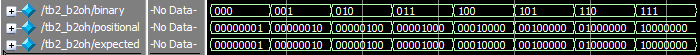
\includegraphics[width=\textwidth]{test2_results}
		\caption{Результаты теста второго класса с вычислением результата}
		\label{fig:test2_results}
	\end{center}
\end{figure}

В листинге \ref{code:test2_error} приведен вывод результатов теста в консоль при внесении ошибки в вычисление ожидаемого значения.
\begin{lstlisting}[caption=Результаты ошибочного теста второго класса с вычислением результата, label=code:test2_error, style=console]
run -all
# 		 time binary positional
#                   40   0     1
#                  120   1     2
# Expected 00000001, got 00000010.
# 
#                  200   2     4
# Expected 00000001, got 00000100.
# 
#                  280   3     8
# Expected 00000001, got 00001000.
# 
#                  360   4    16
# Expected 00000001, got 00010000.
# 
#                  440   5    32
# Expected 00000001, got 00100000.
# 
#                  520   6    64
# Expected 00000001, got 01000000.
# 
#                  600   7   128
# Expected 00000001, got 10000000.
# 
# Testing complited
#    Time: 640 ns  Iteration: 1  Instance: /tb2_b2oh
\end{lstlisting}

\subsection{Тест второго класса с чтением файлов}

В листинге \ref{code:test3} приведено описание теста второго класса с чтением файлов. В данном тесте на вход устройства из файла \code{input_b2oh.dat}, приведенного в листинге \ref{code:input}, подаются всевозможные значения преобразуемого кода, а ожидаемые значения считываются из файла \code{exp_b2oh.dat}, приведенного в листинге \ref{code:exp}. 
\lstinputlisting[caption=\code{tb2f_b2oh.v}, label=code:test3]{tb2f_b2oh.v}

\begin{multicols}{2}
	\lstinputlisting[caption=\code{input_b2oh.dat}, label=code:input, style=dat]{input_b2oh.dat}
	\lstinputlisting[caption=\code{exp_b2oh.dat}, label=code:exp, style=dat]{exp_b2oh.dat}
\end{multicols}

В листинге \ref{code:test3_results} приведен вывод результатов теста в консоль.
\begin{lstlisting}[caption=Результаты теста второго класса с чтением файлов, label=code:test3_results, language={}]
run -all
# 		          time binary positional
#                   80   0     1
#                  160   1     2
#                  240   2     4
#                  320   3     8
#                  400   4    16
#                  480   5    32
#                  560   6    64
#                  640   7   128
# Testing complited
#    Time: 640 ns  Iteration: 1  Instance: /tb2f_b2oh
\end{lstlisting}

На рис. \ref{fig:test3_results} изображена временная диаграмма теста.
\begin{figure}[H]
	\begin{center}
		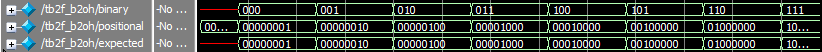
\includegraphics[width=\textwidth]{test3_results}
		\caption{Результаты теста второго класса с чтением файлов}
		\label{fig:test3_results}
	\end{center}
\end{figure}

В листинге \ref{code:test3_error} приведен вывод результатов теста в консоль при внесении ошибок в ожидаемые значения.
\begin{lstlisting}[caption=Результаты ошибочного теста второго класса с чтением файлов, label=code:test3_error, style=console]
run -all
# 		 time binary positional
#                   80   0     1
# Error: expected 10000000, got 00000001.
# 
#                  160   1     2
# Error: expected 00000001, got 00000010.
# 
#                  240   2     4
# Error: expected 00000010, got 00000100.
# 
#                  320   3     8
# Error: expected 00000100, got 00001000.
# 
#                  400   4    16
# Error: expected 00001000, got 00010000.
# 
#                  480   5    32
# Error: expected 00010000, got 00100000.
# 
#                  560   6    64
# Error: expected 00100000, got 01000000.
# 
#                  640   7   128
# Error: expected 01000000, got 10000000.
# 
# Testing complited
#    Time: 640 ns  Iteration: 1  Instance: /tb2f_b2oh
\end{lstlisting}
\vspace{-0.5cm}

\section{Тестирование на плате miniDiLaB\_CIV}

Для тестирования проекта на плате было создано Verilog описание с назначением выходов, приведенное в листинге  \ref{code:dilab}.
\lstinputlisting[caption=\code{dilab_b2oh.v}, label=code:dilab]{dilab_b2oh.v}

Результаты тестирования совпадают с ожидаемыми, следовательно, устройство работает верно.
 
\section{Выводы}

В ходе лабораторной работы на языке Verilog описан параметризированный преобразователь $N$-разрядного двоичного кода в позиционный код. Создано описание тестов первого и второго уровней, а также модуль для проверки работы на плате \code{miniDiLaB_CIV}. Тестирование разработанного устройства показало, что результаты совпадают с ожидаемыми, следовательно устройство работает верно.

\end{document}